\begingroup
\begin{figure}[!htb]
    % \setArraystrech{1.5}
    \centering
    % \setlength\tabcolsep{8pt}
    \begin{tabular*}{\textwidth}{ c c c }
          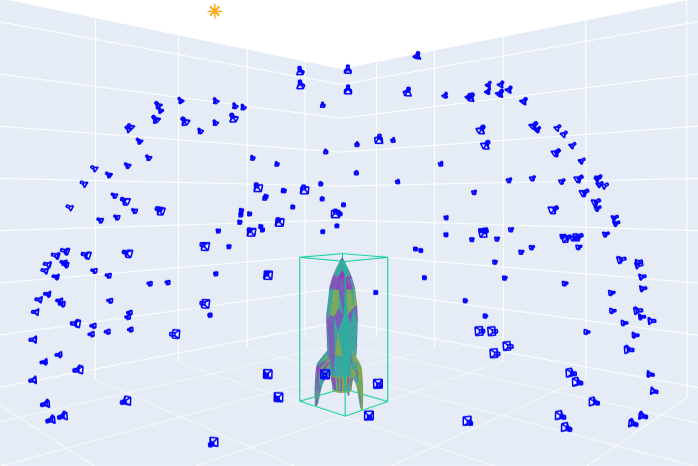
\includegraphics[width=0.32\textwidth]{figures/light_settings/static_setting.png}
        & 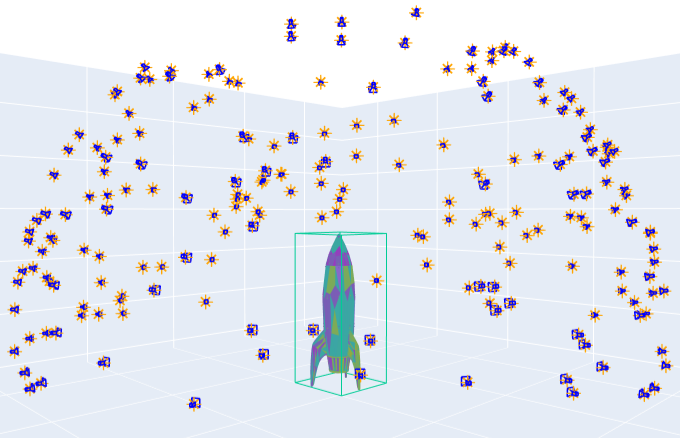
\includegraphics[width=0.29\textwidth]{figures/light_settings/colocated_setting.png}
        & 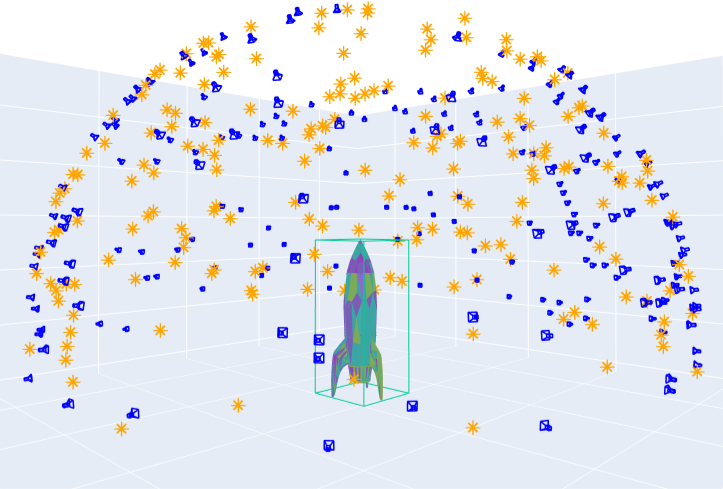
\includegraphics[width=0.29\textwidth]{figures/light_settings/arbitrary_setting.png} \\
        (a) Static & (b) Colocated & (c) Arbitrary
    \end{tabular*}
    \caption{Types of datasets that are used in the experiments.
    Cameras are denoted with blue icons, point light sources are represented by yellow stars.
    In static light setting (a) light source in all of created sample images are placed at the same point
    while camera locations are spread on a clipped sphere around the scene.
    Colocated light setting (b) imply point light sources to be placed at the same position with the camera for each sample view.
    In arbitrary light setting (c) both point light source and camera locations are spread on a clipped spheres around the scene.}
    \label{fig:light_settings}
\end{figure}
\endgroup